\chapter{\sffamily Probabilistic learning algorithms}

{\bfseries\sffamily Concept.} To extend the formalism that we developed in the previous chapter to better understand the time evolution of state probabilities in order to motivate the construction of various learning algorithms. With this knowledge we will see how Gaussian processes and empirical probabilistic reweighting work, as well as discuss how some phenomena permit a convenient description via `mean-field' equations or regression of distribution moments. For the mathematically-inclined, this chapter will take a detailed look at how our formalism can be extended to focus on the time evolution of probabilities, with a view to probabilistic learning later on. For the programmers, this chapter will mostly focus on the algorithm concepts, but all of the relevant software lives in this public Git repository: \href{https://github.com/umbralcalc/learndadex}{https://github.com/umbralcalc/learnadex}.

\section{\sffamily Probabilistic formalism} 

The novelties in this section are less to do with the probabilistic learning methodology and lie more in the specifics of how we combine some of these ideas together when referencing the stochadex formalism, and how this manifests in designing more generally-applicable software for the user. In addition, readers well-versed in machine learning may note that our algorithm designs and mathematical formalism reflect our focus on methods for `online' learning\footnote{We'll explain this later in the chapter.} in the context of time series prediction, in contrast to some of the more standard frameworks.

Let's start by returning to the formalism that we introduced in the previous chapter. As we discussed at that point; this formalism is appropriate for sampling from nearly every stochastic phenomenon that one can think of. We are going to extend this description to consider what happens to the probability that the state history matrix takes a particular set of values over time.

\begin{figure}[h]
\centering
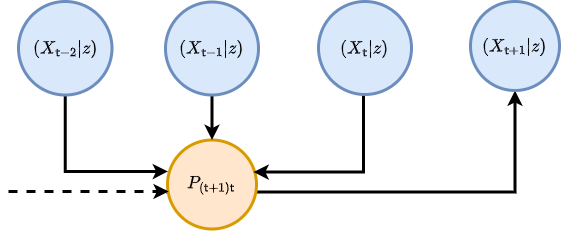
\includegraphics[width=12cm]{images/chapter-2-master-eq-graph.drawio.png}
\caption{Graph representation of Eq.~(\ref{eq:master-x-cont}).}
\label{fig:master-eqn}
\end{figure} 

So, how do we begin? In the first chapter, we defined the general stochastic process with the formula $X^{i}_{{\sf t}+1} = F^{i}_{{\sf t}+1}(X_{0:{\sf t}},z,{\sf t})$. This equation also has an implicit \emph{master equation} associated to it that fully describes the time evolution of the \emph{probability density function} $P_{{\sf t}+1}(X\vert z)$ of $X_{0:{\sf t}+1}=X$ given that the parameters of the process are $z$. This can be written as
%%
\begin{align}
P_{{\sf t}+1}(X\vert z) &= P_{{\sf t}}(X'\vert z) P_{({\sf t}+1){\sf t}}(x\vert X',z) \label{eq:master-x-cont}\,,
\end{align}
%%
where for the time being we are assuming the state space is continuous in each of the matrix elements and $P_{({\sf t}+1){\sf t}}(x\vert X',z)$ is the conditional probability that $X_{{\sf t}+1}=x$ given that $X_{0:{\sf t}}=X'$ at time ${\sf t}$ and the parameters of the process are $z$. To try and understand what Eq.~(\ref{eq:master-x-cont}) is saying, we find it's helpful to think of an iterative relationship between probabilities; each of which is connected by their relative conditional probabilities. We've also illustrated this kind of thinking in Fig.~\ref{fig:master-eqn}.

Consider what happens when we extend the chain of conditional probabilities in Eq.~(\ref{eq:master-x-cont}) back in time by one step. In doing so, we retrieve a joint probability of rows $X_{{\sf t}+1}=x$ and $X_{{\sf t}}=x'$ on the right hand side of the expression 
%%
\begin{align}
P_{{\sf t}+1}(X\vert z) &= P_{{\sf t}-1}(X''\vert z) P_{({\sf t}+1){\sf t}({\sf t}-1)}(x,x'\vert X'',z) \label{eq:master-x-pairwise-joint}\,.
\end{align}
%%
Since Eqs.~(\ref{eq:master-x-cont}) and~(\ref{eq:master-x-pairwise-joint}) are both valid ways to obtain $P_{{\sf t}+1}(X\vert z)$ we can average between them without loss of generality in the original expression, like this
%%
\begin{align}
P_{{\sf t}+1}(X\vert z) &= \frac{1}{2}\big[ P_{{\sf t}}(X'\vert z) P_{({\sf t}+1){\sf t}}(x\vert X',z) + P_{{\sf t}-1}(X''\vert z) P_{({\sf t}+1){\sf t}({\sf t}-1)}(x,x'\vert X'',z) \big]\,.
\end{align}
%%
Following this line of reasoning to its natural conclusion, Eq.~(\ref{eq:master-x-cont}) can hence be generalised to consider all possible joint distributions of rows at different timesteps like this
%%
\begin{align}
P_{{\sf t}+1}(X\vert z) &= \frac{1}{{\sf t}}\sum_{{\sf t}''=0}^{{\sf t}}P_{{\sf t}''}(X''\vert z) P_{({\sf t}+1){\sf t}\dots{\sf t}''}(x,x',\dots \vert X'',z) \label{eq:master-x-cont-sum-gen}\,.
\end{align}
%%

If we wanted to just look at the distribution over the latest row $X_{{\sf t}+1}=x$, we could achieve this through marginalisation over all of the previous matrix rows in Eq.~(\ref{eq:master-x-cont}) like this
%%
\begin{align}
P_{{\sf t}+1}(x\vert z) = \int_{\Omega_{{\sf t}}}{\rm d}X' P_{{\sf t}+1}(X\vert z) &= \int_{\Omega_{{\sf t}}}{\rm d}X' P_{{\sf t}}(X'\vert z) P_{({\sf t}+1){\sf t}}(x\vert X',z) \label{eq:master-x-cont-latest-row} \,.
\end{align}
%%
But what is $\Omega_{\sf t}$? You can think of this as just the domain of possible matrix $X'$ inputs into the integral which will depend on the specific stochastic process we are looking at. 

The symbol ${\rm d}X'$ in Eq.~(\ref{eq:master-x-cont-latest-row}) is our shorthand notation throughout the book for computing the sum of integrals over previous state history matrices which can further be reduced via Eq.~(\ref{eq:master-x-cont-sum-gen}) into a product of sub-domain integrals over each matrix row
%%
\begin{align}
P_{{\sf t}+1}(x\vert z) &= \frac{1}{{\sf t}}\sum_{{\sf t}''=0}^{{\sf t}} \bigg\lbrace \int_{\omega_{{\sf t}'}}{\rm d}^nx'...\int_{\Omega_{{\sf t}''}}{\rm d}X'' \bigg\rbrace \,P_{{\sf t}''}(X''\vert z) P_{({\sf t}+1){\sf t}\dots{\sf t}''}(x,x',... \vert X'',z) \\
&= \frac{1}{{\sf t}}\sum_{{\sf t}''=0}^{{\sf t}} \int_{\Omega_{{\sf t}''}}{\rm d}X'' P_{{\sf t}''}(X''\vert z) P_{({\sf t}+1){\sf t}''}(x \vert X'',z) \label{eq:master-x-cont-latest-row-gen} \,,
\end{align}
%%
where each row measure is a Cartesian product of $n$ elements (a Lebesgue measure), i.e.,
%%
\begin{align}
{\rm d}^nx = \prod_{i=0}^n{\rm d}x^i \,,
\end{align}
%%
and lowercase $x, x', \dots$ values will always refer to individual rows within the state matrices. Note that $1/{\sf t}$ here is a normalisation factor --- this just normalises the sum of all probabilities to 1 given that there is a sum over ${\sf t}'$. Note also that, if the process is defined over continuous time, we would need to replace 
%%
\begin{align}
\frac{1}{{\sf t}}\sum_{{\sf t}'=0}^{{\sf t}} \rightarrow \frac{1}{t({\sf t})}\sum_{{\sf t}'=0}^{{\sf t}}\delta t({\sf t}') \,.
\end{align}
%%

Let's go through some examples. Non-Markovian phenomena with continuous state spaces can have quite complex master equations. A relatively simple example is that of pure diffusion processes which exhibit stochastic resetting at a rate $r$ to a remembered location from the trajectory history~\cite{boyer2017long}
%%
\begin{align}
P_{{\sf t}+1}(x\vert z) &= (1-r)P_{{\sf t}}(x\vert z) + \sum_{i=0}^n\sum_{j=0}^n\frac{\partial}{\partial x^i}\frac{\partial}{\partial x^j}\bigg[ D_{{\sf t}}(x,z)P_{{\sf t}}(x\vert z) \bigg] + r\sum_{{\sf t}'=0}^{{\sf t}}\delta t ({\sf t}')K[t({\sf t}){-}t({\sf t}')]P_{{\sf t}'}(x\vert z) \,,
\end{align}
%%
where here $K$ is some memory kernel. For Markovian phenomena which have a continuous state space, Eqs.~(\ref{eq:master-x-cont}) and~(\ref{eq:master-x-cont-latest-row}) no longer depend on timesteps older than the immediately previous one, hence, e.g., Eq.~(\ref{eq:master-x-cont-latest-row}) reduces to just
%%
\begin{align}
P_{{\sf t}+1}(x\vert z) &= \int_{\omega_{\sf t}}{\rm d}^nx' \, P_{\sf t}(x'\vert z) P_{({\sf t}+1){\sf t}}(x\vert x',z) \label{eq:master-x-cont-markov} \,.
\end{align}
%%
A famous example of this kind of phenomenon arises from approximating Eq.~(\ref{eq:master-x-cont-markov}) with an expansion (Kramers-Moyal~\cite{kramers1940brownian, moyal1949stochastic}) up to second-order, yielding the Fokker-Planck equation 
%%
\begin{align}
P_{{\sf t}+1}(x\vert z) &= P_{{\sf t}}(x\vert z) - \sum_{i=0}^n\frac{\partial}{\partial x^i}\bigg[ \mu_{{\sf t}}(x,z)P_{{\sf t}}(x\vert z)\bigg] + \sum_{i=0}^n\sum_{j=0}^n\frac{\partial}{\partial x^i}\frac{\partial}{\partial x^j}\bigg[ D_{{\sf t}}(x,z)P_{{\sf t}}(x\vert z) \bigg] \,,
\end{align}
%%
which describes a process undergoing drift-diffusion.

An analog of Eq.~(\ref{eq:master-x-cont-latest-row}) exists for discrete state spaces as well. We just need to replace the integral with a sum and the schematic would look something like this
%%
\begin{align}
P_{{\sf t}+1}(x\vert z) &= \sum_{\Omega_{{\sf t}}} P_{{\sf t}}(X'\vert z) P_{({\sf t}+1){\sf t}}(x \vert X', z) \label{eq:master-x-disc} \,,
\end{align}
%%
where we note that the $P$'s in the expression above all now refer to \emph{probability mass functions}. In what follows, discrete state space can always be considered by replacing the integrals with summations over probability masses in this manner; we only use the continuous state space formulation for our notation because one could argue it's a little more general. 

Analogously to continuous state spaces, we can give some examples of master equations for phenomena with a discrete state space as well. In the Markovian case, we need look no further than a simple time-dependent Poisson process
%%
\begin{align}
P_{{\sf t}+1}(x\vert z) &= \lambda ({\sf t}) \delta t({\sf t}{+}1)P_{{\sf t}}(x{-}1\vert z) + \big[1-\lambda ({\sf t}) \delta t({\sf t}{+}1)\big] P_{{\sf t}}(x\vert z) \,.
\end{align}
%%
For such an example of a non-Markovian system, a Hawkes process~\cite{hawkes1971spectra} master equation would look something like this
%%
\begin{align}
P_{{\sf t}+1}(x\vert z) &= \mu \delta t({\sf t}{+}1)P_{{\sf t}}(x{-}1\vert z) + \big[ 1-\mu \delta t({\sf t}{+}1)\big] P_{{\sf t}}(x\vert z) \nonumber \\
& + \sum_{x'=0}^\infty\sum_{{\sf t}'=0}^{{\sf t}} \phi [t({\sf t})-t({\sf t}')] \delta t({\sf t}{+}1)P_{{\sf t}{\sf t}'({\sf t}'-1)}(x{-}1,x',x'{-}1\vert z) \nonumber \\
&+ \sum_{x'=0}^\infty\bigg\lbrace 1-\sum_{{\sf t}'=0}^{{\sf t}} \phi [t({\sf t})-t({\sf t}')] \delta t({\sf t}{+}1)\bigg\rbrace P_{{\sf t}{\sf t}'({\sf t}'-1)}(x, x', x'{-}1\vert z) \,,
\end{align}
%%
where we note the complexity in this expression arises because it has to include a coupling between the rate at which events occur and an explicit memory of when the previous ones did occur (recorded by differencing the count between adjacent timesteps by 1).

\section{\sffamily Motivating the algorithms}

So now that we are more familiar with the notation used by Eq.~(\ref{eq:master-x-cont-latest-row}), we can use it to motivate and derive some useful learning algorithms. While it's worth going into some mathematical detail to give a better sense of where each technique comes from, we should emphasise that the methodologies we discuss here are not new to the technical literature at all. We draw on influences from Empirical Dynamical Modeling (EDM)~\cite{sugihara1990nonlinear}, some classic nonparametric local regression techniques --- such as LOWESS/Savitzky-Golay filtering~\cite{savitzky1964smoothing} --- and also Gaussian processes~\cite{murphy2012machine}.  

Let's begin our discussion of algorithms by integrating Eq.~(\ref{eq:master-x-cont-latest-row}) over $x$ to obtain a relation for the mean of the distribution
%%
\begin{align}
M_{{\sf t}+1}(z) &= \int_{\omega_{{\sf t}+1}}{\rm d}^nx \,x\, P_{{\sf t}+1}(x\vert z) = \frac{1}{{\sf t}}\sum_{{\sf t}''=0}^{{\sf t}} \int_{\Omega_{{\sf t}''}}{\rm d}X'' P_{{\sf t}''}(X''\vert z) M_{({\sf t}+1){\sf t}''}(X'',z) \label{eq:mean-field-master}\,,
\end{align}
%%
where you can view the $M_{({\sf t}+1){\sf t}''}(X'',z)$ values as either terms in some regression model, or derivable explicitly from a known master equation. The latter of these provides one approach to statistically infer the states and parameters of stochastic simulations from data: one begins by knowing what the master equation is, uses this to compute the time evolution of the mean (and potentially higher-order statistics) and then connects these ${\sf t}$ and $z$-dependent statistics back to the likelihood of observing the data. This is what is commonly known as the `mean-field' inference approach; averaging over the available degrees of freedom in the statistical moments of distributions. Though, knowing what the master equation is for an arbitrarily-defined stochastic phenomenon can be very difficult indeed, and the resulting equations typically require some form of approximation. 

\begin{figure}[h]
\centering
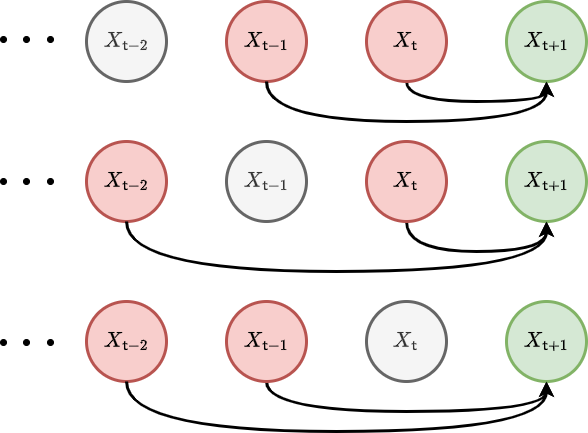
\includegraphics[width=8cm]{images/chapter-2-second-temporal-correlation.drawio.png}
\caption{A graph representation of the correlations in Eq.~(\ref{eq:second-order-correl}).}
\label{fig:second-temporal-correlation}
\end{figure} 

Given that the mean-field approach isn't always going to be viable as an inference method, we should also consider other ways to describe the shape and time evolution characteristics of $P_{{\sf t}+1}(X\vert z)$. For continuous state spaces, it's possible to approximate this whole distribution with a logarithmic expansion like so
%%
\begin{align}
\ln P_{{\sf t}+1}(X\vert z) &\simeq \ln P_{{\sf t}+1}(X_*\vert z) + \frac{1}{2}\sum_{{\sf t}'=0}^{{\sf t}+1}\sum_{i=0}^{n}\sum_{j=0}^{n} (x-x_*)^i {\cal H}^{ij}_{({\sf t}+1){\sf t}'}(x_*,x'_*) (x'-x'_*)^j \label{eq:second-order-log-expansion} \\
{\cal H}^{ij}_{({\sf t}+1){\sf t}'}(x_*,x'_*) &= \frac{\partial}{\partial x^i}\frac{\partial}{\partial (x')^j}\ln P_{{\sf t}+1}(X\vert z) \bigg\vert_{X=X_*} \,,
\end{align}
%% 
where the values for $X=X_*$ are defined by the vanishing of the first derivative, i.e., these are chosen such that
%%
\begin{align}
\frac{\partial}{\partial x^i}\ln P_{{\sf t}+1}(X\vert z) \bigg\vert_{X=X_*} &= 0 \,.
\end{align}
%%
If we keep the truncation up to second order in Eq.~(\ref{eq:second-order-log-expansion}), note that this expression implies a pairwise correlation structure of the form
%%
\begin{align}
P_{{\sf t}+1}(X\vert z) &\rightarrow \prod_{{\sf t}'=0}^{{\sf t}}P_{({\sf t}+1){\sf t}'}(x,x'\vert z) = \prod_{{\sf t}'=0}^{{\sf t}}P_{{\sf t}'}(x'\vert z)P_{({\sf t}+1){\sf t}'}(x\vert x', z) \,.
\end{align}
%%
Given this pairwise temporal correlation structure, Eq.~(\ref{eq:master-x-cont-latest-row-gen}) reduces to this simpler sum of integrals
%%
\begin{align}
P_{{\sf t}+1}(x\vert z) &= \frac{1}{{\sf t}}\sum_{{\sf t}'=0}^{{\sf t}}\int_{\omega_{{\sf t}'}}{\rm d}^nx' P_{{\sf t}'}(x'\vert z)P_{({\sf t}+1){\sf t}'}(x\vert x',z) \label{eq:second-order-correl} \,.
\end{align}
%%
We have illustrated these second-order correlations with a graph visualisation in Fig.~(\ref{fig:second-temporal-correlation}).

\begin{figure}[h]
\centering
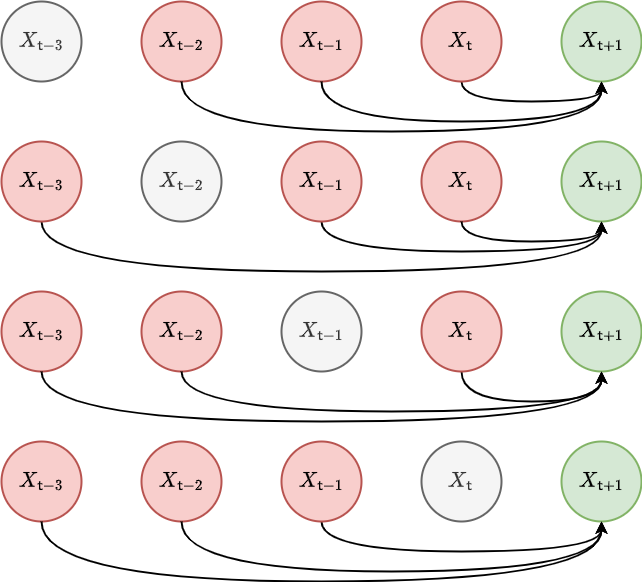
\includegraphics[width=10cm]{images/chapter-2-third-temporal-correlation.drawio.png}
\caption{A graph representation of the correlations in Eq.~(\ref{eq:third-order-correl}).}
\label{fig:third-temporal-correlation}
\end{figure}

In a similar fashion, we can increase the expansion order of Eq.~(\ref{eq:second-order-log-expansion}) to include third-order correlations such that 
%%
\begin{align}
P_{{\sf t}+1}(X\vert z) &\rightarrow \prod_{{\sf t}'=0}^{{\sf t}}\prod_{{\sf t}''=0}^{{\sf t}'-1} P_{{\sf t}'{\sf t}''}(x',x''\vert z)P_{({\sf t}+1){\sf t}'{\sf t}''}(x\vert x',x'',z) \,,
\end{align}
%%
and, in this instance, one can show that Eq.~(\ref{eq:master-x-cont-latest-row-gen}) reduces to
%%
\begin{align}
P_{{\sf t}+1}(x\vert z) &= \frac{1}{{\sf t}}\sum_{{\sf t}'=0}^{{\sf t}}\frac{1}{{\sf t}'-1}\sum_{{\sf t}''=0}^{{\sf t}'-1}\int_{\omega_{{\sf t}'}}{\rm d}^nx'\int_{\omega_{{\sf t}''}}{\rm d}^nx'' P_{{\sf t}'{\sf t}''}(x',x''\vert z)P_{({\sf t}+1){\sf t}'{\sf t}''}(x\vert x',x'',z) \label{eq:third-order-correl} \,.
\end{align}
%%
We have also illustrated these third-order correlations with another graph visualisation in Fig.~(\ref{fig:third-temporal-correlation}). Using $P_{{\sf t}'{\sf t}''}(x',x''\vert z) = P_{{\sf t}''}(x''\vert z) P_{{\sf t}'{\sf t}''}(x'\vert x'', z)$ one can also show that this integral is a marginalisation of this expression
%%
\begin{align}
P_{({\sf t}+1){\sf t}''}(x\vert x'', z) &= \frac{1}{{\sf t}}\sum_{{\sf t}'=0}^{{\sf t}}\int_{\omega_{{\sf t}'}}{\rm d}^nx'P_{{\sf t}'{\sf t}''}(x'\vert x'',z)P_{({\sf t}+1){\sf t}'{\sf t}''}(x\vert x',x'',z) \,,
\end{align}
%%
which describes the time evolution of the conditional probabilities.

Another probabilistic learning algorithm that we can derive is what we shall call `empirical probabilistic reweighting'. There is another expression for the mean of the distribution, that we can derive under certain conditions, which will be valuable to motivating this algorithm. If the probability distribution over each row of the state history matrix is \emph{stationary} --- meaning that $P_{{\sf t}+1}(x\vert z)=P_{{\sf t}'}(x\vert z)$ --- it's possible to go one step further than Eq.~(\ref{eq:mean-field-master}) and assert that
%%
\begin{align}
M_{{\sf t}+1}(z) &= \int_{\omega_{{\sf t}+1}}{\rm d}^nx \,x\,P_{{\sf t}+1}(x\vert z) = \frac{1}{{\sf t}}\sum_{{\sf t}'=0}^{{\sf t}}\int_{\omega_{{\sf t}'}}{\rm d}^nx' \,x'\, P_{{\sf t}'}(x'\vert z) \int_{\omega_{{\sf t}+1}}{\rm d}^nx\, P_{({\sf t}+1){\sf t}'}(x\vert x',z) \label{eq:stationary-mean-estimator}\,.
\end{align}
%%

To see that Eq.~(\ref{eq:stationary-mean-estimator}) is true, first note that a joint distribution over both $x$ and $x'$ can be derived like this $P_{({\sf t}+1){\sf t}'}(x,x'\vert z)=P_{({\sf t}+1){\sf t}'}(x\vert x',z)P_{{\sf t}'}(x'\vert z)$. Secondly, note that this joint distribution will always allow variable swaps trivially like this $P_{({\sf t}+1){\sf t}'}(x,x'\vert z)=P_{{\sf t}'({\sf t}+1)}(x',x\vert z)$. Then, lastly, note that stationarity of $P_{{\sf t}+1}(x\vert z)=P_{{\sf t}'}(x\vert z)$ means 
%%
\begin{align}
\frac{1}{{\sf t}}\sum_{{\sf t}'=0}^{{\sf t}}\int_{\omega_{{\sf t}+1}} {\rm d}^nx\int_{\omega_{{\sf t}'}} {\rm d}^nx' \,x\, P_{({\sf t}+1){\sf t}'}(x,x'\vert z)&=\frac{1}{{\sf t}}\sum_{{\sf t}'=0}^{{\sf t}}\int_{\omega_{{\sf t}'}} {\rm d}^nx\int_{\omega_{{\sf t}+1}} {\rm d}^nx' \,x\, P_{{\sf t}'({\sf t}+1)}(x,x'\vert z)\nonumber \\
&=\frac{1}{{\sf t}}\sum_{{\sf t}'=0}^{{\sf t}}\int_{\omega_{{\sf t}'}} {\rm d}^nx'\int_{\omega_{{\sf t}+1}} {\rm d}^nx \,x'\, P_{({\sf t}+1){\sf t}'}(x,x'\vert z) \nonumber \\
&=\frac{1}{{\sf t}}\sum_{{\sf t}'=0}^{{\sf t}}\int_{\omega_{{\sf t}'}}{\rm d}^nx' \,x'\, P_{{\sf t}'}(x'\vert z) \int_{\omega_{{\sf t}+1}}{\rm d}^nx\, P_{({\sf t}+1){\sf t}'}(x\vert x',z)\nonumber \,,
\end{align}
%%
where we've used the trivial variable swap and integration variable relabelling to arrive at the second equality in the expressions above. 

The standard covariance matrix elements can also be computed in a similar fashion
%%
\begin{align}
C^{ij}_{{\sf t}+1}(z) &= \int_{\omega_{{\sf t}+1}}{\rm d}^nx \,[x-M_{{\sf t}+1}(z)
]^i[x-M_{{\sf t}+1}(z)]^jP_{{\sf t}+1}(x\vert z) \nonumber \\
&= \frac{1}{{\sf t}}\sum_{{\sf t}'=0}^{{\sf t}}\int_{\omega_{{\sf t}'}}{\rm d}^nx' \, [x'-M_{{\sf t}+1}(z)]^i[x'-M_{{\sf t}+1}(z)]^j \,P_{{\sf t}'}(x'\vert z) \int_{\omega_{{\sf t}+1}}{\rm d}^nx \, P_{({\sf t}+1){\sf t}'}(x\vert x',z) \label{eq:stationary-covariance-estimator}\,.
\end{align}
%%
While they look quite abstract, Eqs.~(\ref{eq:stationary-mean-estimator}) and~(\ref{eq:stationary-covariance-estimator}) express the core idea behind how the probabilistic reweighting will function. By assuming a stationary distribution, we gain the ability to directly estimate the statistics of the probability distribution of the next sample from the stochastic process $P_{{\sf t}+1}(x\vert z)$ from past samples it may have in empirical data; which are represented here by $P_{{\sf t}'}(x'\vert z)$. More on this later.

\section{\sffamily Learning algorithms}

Probabilistic reweighting depends on the stationarity of $P_{{\sf t}+1}(x\vert z)=P_{{\sf t}'}(x\vert z)$ such that, e.g., Eq.~(\ref{eq:stationary-mean-estimator}) is applicable. The core idea behind it is to represent the past distribution of state values $P_{{\sf t}'}(x'\vert z)$ with the samples from a real time series dataset. If the user then specifies a good model for the relationships in this data by providing a weighting function which returns the conditional probability mass
%%
\begin{align}
{\sf w}_{{\sf t}'}(y,z) = \int_{\omega_{{\sf t}+1}} {\rm d}^nx \, P_{({\sf t}+1){\sf t}'}(x\vert x'{=}y,z) \,,  
\end{align}
%%
we can apply this as a \emph{reweighting} of the historical time series samples to estimate any statistics of interest. Taking Eqs.~(\ref{eq:stationary-mean-estimator}) and~(\ref{eq:stationary-covariance-estimator}) as the examples; we are essentially approximating these integrals through weighted sample estimations like this
%%
\begin{align}
M_{{\sf t}+1}(z) &\simeq \frac{1}{{\sf t}}\sum^{{\sf t}}_{{\sf t}'=0}Y_{{\sf t}'} {\sf w}_{{\sf t}'}(Y_{{\sf t}'},z) \label{eq:mean-reweighting} \\
C^{ij}_{{\sf t}+1}(z) &\simeq \frac{1}{{\sf t}}\sum^{{\sf t}}_{{\sf t}'=0}[Y_{{\sf t}'}-M_{{\sf t}+1}(z)]^i[Y_{{\sf t}'}-M_{{\sf t}+1}(z)]^j \, {\sf w}_{{\sf t}'}(Y_{{\sf t}'},z) \label{eq:covariance-reweighting} \,,
\end{align}
%%
where we have defined the data matrix $Y$ with rows $Y_{{\sf t}+1}, Y_{{\sf t}}, \dots$, each of which representing specific observations of the rows in $X$ at each point in time from a real dataset.

The goal of a learning algorithm for probabilistic reweighting would be to learn the optimal reweighting function ${\sf w}_{{\sf t}'}(Y_{{\sf t}'},z)$ with respect to $z$, i.e., the ones which most accurately represent a provided dataset. But before we think about the various kinds of conditional probability we could use, we need to think about how to connect the post-reweighting statistics to the data by defining an objective function. 

If the mean is a sufficient statistic for the distribution which describes the data, a choice of, e.g., Exponential, Poisson or Binomial distribution could be used where the mean is estimated directly from the time series using Eq.~(\ref{eq:stationary-mean-estimator}), given a conditional probability $P_{({\sf t}+1){\sf t}'}(x\vert x',z)$. Extending this idea further to include distributions which also require a variance to be known, e.g., the Normal, Gamma or Negative Binomial distributions could be used where the variance (and/or covariance) could be estimated using Eq.~(\ref{eq:stationary-covariance-estimator}). These are just a few simple examples of distributions that can link the estimated statistics from Eqs.~(\ref{eq:stationary-mean-estimator}) and~(\ref{eq:stationary-covariance-estimator}) to a time series dataset. However, the algorithmic framework is very general to whatever choice of `data linking' distribution that a researcher might need.

We should probably make what we've just said a little more mathematically concrete. We can define $P_{{\sf t}+1}[y;M_{{\sf t}+1}(z),C_{{\sf t}+1}(z),\dots ]$ as representing the likelihood of $y = Y_{{\sf t}+1}$ given the estimated statistics from Eqs.~(\ref{eq:stationary-mean-estimator}) and~(\ref{eq:stationary-covariance-estimator}) (and maybe higher-orders). Note that in order to do this, we need to identify the $x'$ and ${\sf t}'$ values that are used to estimate, e.g., $M_{{\sf t}+1}(z)$ with the past data values which are observed in the dataset time series itself. Now that we have this likelihood, we can immediately evaluate an objective function (a cumulative log-likelihood) that we might seek to optimise over for a given dataset 
%%
\begin{align}
\ln {\cal L}_{{\sf t}+1}(Y\vert z) &= \sum_{{\sf t}'=0}^{{\sf t}+1} \ln P_{{\sf t}'}[y;M_{{\sf t}'}(z),C_{{\sf t}'}(z),\dots ] \,, \label{eq:log-likelihood-reweighting}
\end{align}
%%
where the summation continues until all of the past measurements $Y_{{\sf t}+1}, Y_{{\sf t}}, \dots$ which exist as rows in the data matrix $Y$ have been taken into account. The code to compute this objective function follows the schematic we have provided in Fig.~\ref{fig:prob-reweighting-code}.

\begin{figure}[h]
\centering
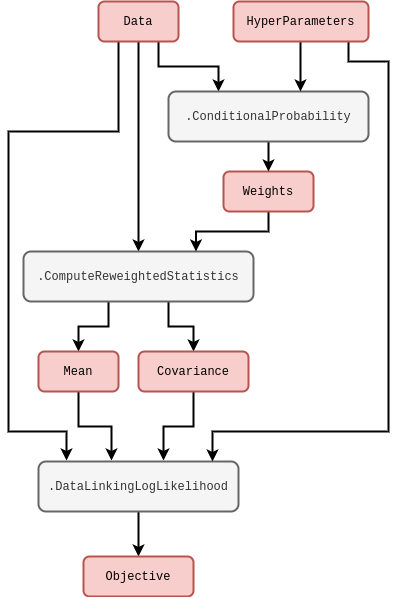
\includegraphics[width=8cm]{images/chapter-2-prob-reweighting-code.drawio.png}
\caption{Code schematic of the probability reweighting optimisation.}
\label{fig:prob-reweighting-code}
\end{figure} 

In order to specify what $P_{({\sf t}+1){\sf t}'}(x\vert x',z)$ is, it's quite natural to define a set of hyperparameters for the elements of $z$. To get a sense of how the data-linking function relates to these hyperparameters, it's instructive to consider an example. One generally-applicable option for the conditional probability could be a purely time-dependent kernel
%%
\begin{align}
P_{({\sf t}+1){\sf t}'}(x\vert x',z) &\propto {\cal K}(z, {\sf t}+1,{\sf t}')  \label{eq:time-dependent-kernel} \,, 
\end{align}
%%
and the data-linking distribution, e.g., could be a Gaussian
%%
\begin{align}
P_{{\sf t}+1}[y;M_{{\sf t}+1}(z),C_{{\sf t}+1}(z),\dots ] = {\sf MultivariateNormalPDF}[y;M_{{\sf t}+1}(z),C_{{\sf t}+1}(z)] \label{eq:gaussian-data-prob}\,.
\end{align}
%%
It's worth pointing out that other machine learning frameworks could easily be used to model these conditional probabilities. For example, neural networks could be used to infer the optimal reweighting scheme and this would still allow us to use the data-linking distribution.\footnote{One can think of using this neural network-based reweighting scheme as similar to constructing a normalising flow model~\cite{kobyzev2020normalizing} with an autoregressive layer. Invertibility and further network structural constraints mean that these are not exactly equivalent, however.} It would still be desirable to keep the data-linking distribution as it can usually be sampled from very easily --- something that can be quite difficult to achieve with a purely machine learning-based representation of the distribution. Sampling itself could even be made more flexible by leveraging a Variational Autoencoder (VAE)~\cite{pinheiro2021variational}; these use neural networks not just on the compression (or `encode') step to estimate the statistics but also use them as a layer between the sample from the data distribution model and the output (the `decode' step).

In the case of Eqs.~(\ref{eq:time-dependent-kernel}) and~(\ref{eq:gaussian-data-prob}) above, the hyperparameters that would be optimised could relate to the kernel in a wide variety of ways. Optimising them would make our optimised reweighting very similar to (but not quite the same as) evaluating maximum a posteriori (MAP) of a Gaussian process regression. The main differences here are that the mean of a Gaussian process as a function of time is typically included within $z$, and hence must be obtained through optimisation. In contrast, our methodology relies on the fact that the mean estimator can be computed directly by weighted sample estimation and can then be fed to some data-linking distribution. 

\textcolor{red}{Got to here in rewrite... Need to talk about the same as above for Gaussian process regression.}

The optimisation approach that we choose to use for obtaining the best hyperparameters in the conditional probability of Eq.~(\ref{eq:log-likelihood-reweighting}) will depend on a few factors. For example, if the number of hyperparameters is relatively low, but their gradients are difficult to calculate exactly; then a gradient-free optimiser (such as the Nelder-Mead~\cite{nelder1965simplex} method or something like a particle swarm~\cite{kennedy1995particle, shi1998modified}) would likely be the most effective choice. On the other hand, when the number of hyperparameters ends up being relatively large, it's usually quite desriable to utilise the gradients in algorithms like vanilla Stochastic Gradient Descent~\cite{robbins1951stochastic} (SGD) or Adam~\cite{kingma2014adam}.

If the gradients of Eq.~(\ref{eq:log-likelihood-reweighting}) are needed, we can always factorise each derivative with respect to hyperparameter $z^i$ in the following way through the chain rule
%%
\begin{align}
\frac{\partial}{\partial z^i}\ln {\cal L}_{{\sf t}+1}(Y \vert z) &= \sum_{{\sf t}'=0}^{{\sf t}+1}\frac{\partial M_{{\sf t}'}}{\partial z^i}\frac{\partial}{\partial M_{{\sf t}'}}\ln P_{{\sf t}'}[y;M_{{\sf t}'}(z),C_{{\sf t}'}(z),\dots ] \nonumber \\
&\qquad + \sum_{{\sf t}'=0}^{{\sf t}+1}\frac{\partial C_{{\sf t}'}}{\partial z^i}\frac{\partial }{\partial C_{{\sf t}'}}\ln P_{{\sf t}'}[y;M_{{\sf t}'}(z),C_{{\sf t}'}(z),\dots ] \,. \label{eq:log-likelihood-reweighting-grad}
\end{align}
%%
By factoring derivatives in this manner, the computation can be separated into two parts: the derivatives with respect to $M_{{\sf t}'}$ and $C_{{\sf t}'}$, which are typically quite straightforward; and the derivatives with respect to $z$ elements, which typically need a more involved calculation depending on the model. Incidentally, this separation also neatly lends itself to abstracting gradient calculations as having a simpler, general purpose component that can be built directly into a library of data models and a more complex, model-specific component that the user must specify.

    